\chapter{Testing} % (fold)
\label{cha:testing}

\section{Unit Test, Integration Test and System Test} % (fold)
\label{sec:unit_test_integration_test_and_system_test}
	
	All the modules are tested individually in separate Xcode project, and integrated into our main project \emph{Fancy Foodie} afterwards. After making sure the features are integrated with the main project, we build the project nightly, and test the function systematically with both simulators and real cellphone whose model is iPhone 5.
% section unit_test_integration_test_and_system_test (end)

\section{Beta Testing} % (fold)
\label{sec:beta_testing}

	\emph{Fancy Foodie} use TestFlight to do beta testing on the fly. TestFlight provides a SDK for us to integrate it to the app. After integration, crash reporting will happen automatically. By logging in the dashboard of TestFlight, we could see all the information for each session of users as shown in Figure~\ref{fig:testflight-dashboard}.

\begin{figure}
	\centering
    \SetFigLayout{1}{1}
    {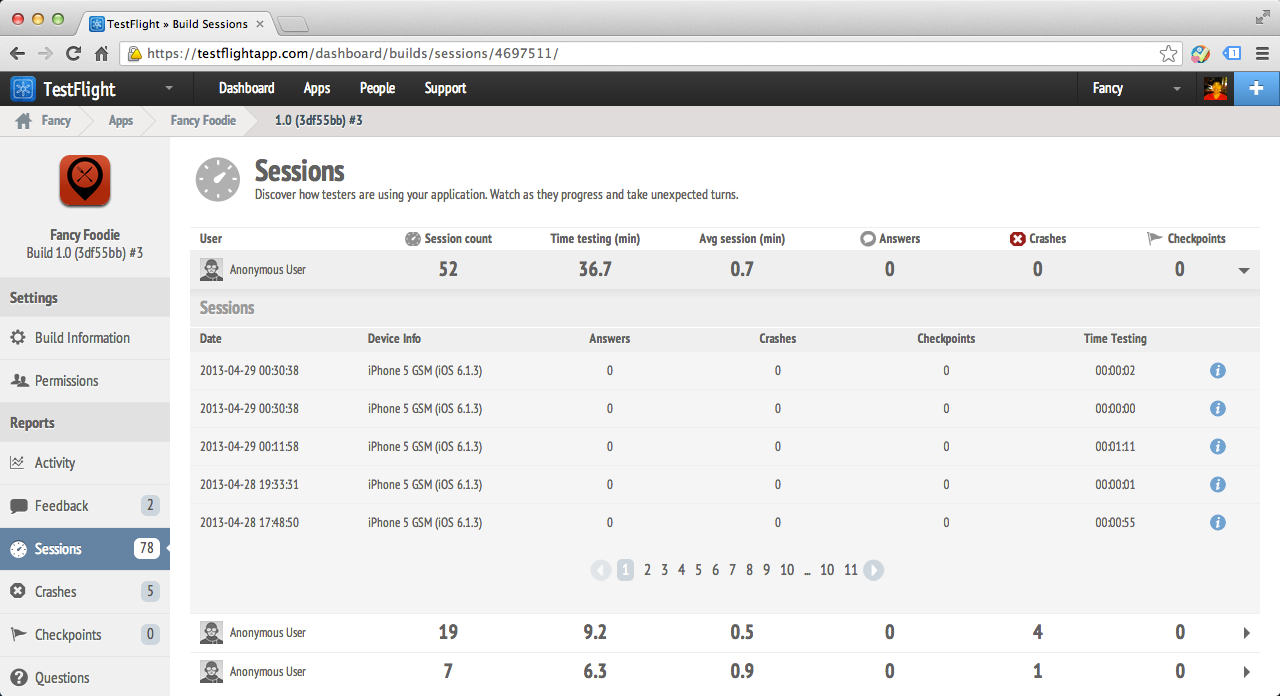
\includegraphics[%
    width=\figwidth, totalheight=\figheight, keepaspectratio]{./screenshots/testflight-dashboard.png}}
    \caption{TestFlight Dashboard}
	\label{fig:testflight-dashboard}
\end{figure}

% section beta_testing (end)

\section{iTunes} % (fold)
\label{sec:itunes}

	\emph{Fancy Foodie} is created in iTunes Connect on April 17, 2013. First submission was uploaded on April 17, 2013. But minor changes are made after that, so another submission was upload on April 23, 2013. Currently, \emph{Fancy Foodie} is waiting for review. After review, https://itunes.apple.com/us/app/fancy-foodie/id638036832?ls=1&mt=8 should be available to U.S. users. Anyone could download the App via that link.
% section itunes (end)

\section{Future Testing} % (fold)
\label{sec:future_testing}

Since it is ongoing project, future testing will be done by using TestFlight as well. We would set up checkpoint and create questionnaire to get better feedback from users. 
% section future_testing (end)
% chapter testing (end)